\documentclass[../main.tex]{subfiles}

\begin{document}

\section{Plateas}

\href{https://youtu.be/-qSCiId3S-c}{Link a clase.}

\subsection{Repaso teorico: coeficiente de balasto}

La teoría del coeficiente de balasto se basa en que las tensiones son proporcionales
a las deformaciones, es decir:

\begin{align*}
  P = k * y 
.\end{align*}

\begin{figure}[ht]
  \centering
  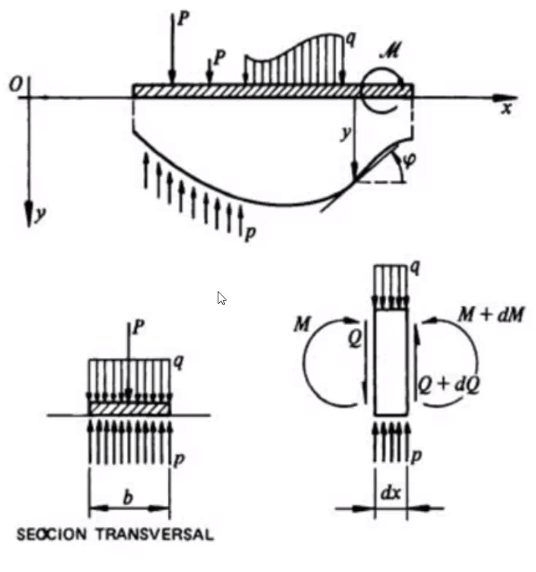
\includegraphics[width=0.4\textwidth]{../images/20210421/balasto}
  \caption{Esquemas de cargas}
  \label{fig:balasto}
\end{figure}

Encontramos las cargas dadas segun el cuadro elemental de la imagen. Desarrollando
la expresión de Navier-Bernoulli, podemos encontrar lo siguiente:

\begin{align*}
  M &= -EI * \frac{\partial^2 y}{\partial x^2} \\[5pt]
  EI \frac{\partial^4 y}{\partial x^4} +b*k_s*y &= b*q 
.\end{align*}

Donde la \textit{longitud elástica} es la siguiente:

\begin{align*}
  L = \left( \frac{4 * E * I}{b * k_s} \right)^{\frac{1}{4}}
.\end{align*}

Finalmente, podemos dejar la ecuación diferencial como:

\begin{align*}
  \frac{\partial^4 y}{\partial \epsilon^4} + 4 * y = \frac{4}{k_s}*q
.\end{align*}

\clearpage
\subsection{Ejercicio 1 de plateas}

\begin{figure}[ht]
  \centering
  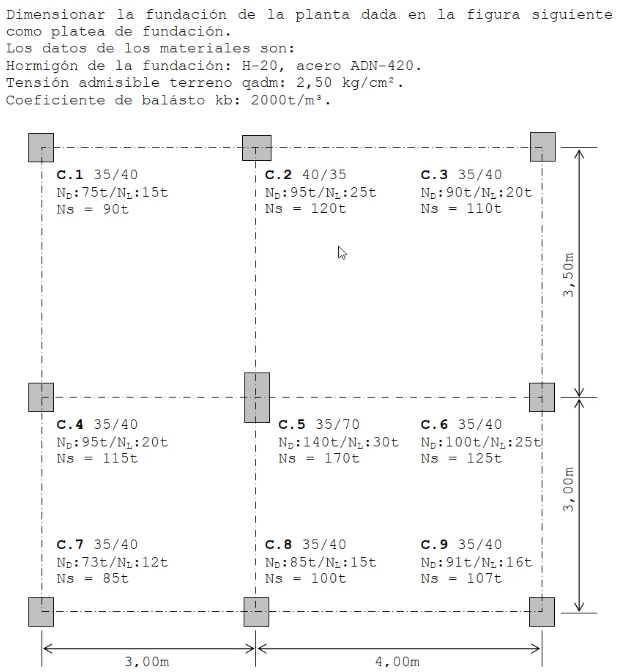
\includegraphics[width=0.8\textwidth]{../images/20210421/ej1}
\end{figure}

Lo primero que podemos requerer es el área necesaria, que será:

\begin{align*}
  A_{nec}=\frac{1.1*N_s}{q_{adm}}
.\end{align*}

Lo que ocurrirá normalmente es además que no se encuentre la carga en el medio,
por lo que la traslación del esfuerzo normal generará un \textit{momento}.

Definimos como $L_x = \SI{7}{m}$ y $L_y = \SI{6.5}{m}$. Sumando todas las cargas
de servicio podemos encontrar lo siguiente:

\begin{align*}
  R_s = \Sigma N_s = \SI{1022}{tn}
.\end{align*}

Luego, encontramos los centros de gravedad simplemente de la siguiente forma.

\begin{align*}
  X_{CG} = \frac{\Sigma (N_s * Y_i)}{R_s} = \SI{3.4873}{m} \\[5pt]
  Y_{CG} = \frac{\Sigma (N_s * Y_i)}{R_s} = \SI{3.2387}{m}
.\end{align*}

O resolviendo en Excel:

% Table generated by Excel2LaTeX from sheet 'Hoja1'
\begin{table}[htbp]
  \centering
  \caption{Cálculo de baricentro}
    \begin{tabular}{|l|r|rrrr}
    \hline
    \rowcolor[rgb]{ .851,  .851,  .851} \textbf{Columna} & \multicolumn{1}{l|}{\textbf{Ns}} & \multicolumn{1}{l|}{\textbf{X}} & \multicolumn{1}{l|}{\textbf{Y}} & \multicolumn{1}{l|}{\textbf{N*X}} & \multicolumn{1}{l|}{\textbf{N*Y}} \bigstrut\\
    \hline
    C1    & 90    & \multicolumn{1}{r|}{0} & \multicolumn{1}{r|}{6.5} & \multicolumn{1}{r|}{0} & \multicolumn{1}{r|}{585} \bigstrut\\
    \hline
    C2    & 120   & \multicolumn{1}{r|}{3} & \multicolumn{1}{r|}{6.5} & \multicolumn{1}{r|}{360} & \multicolumn{1}{r|}{780} \bigstrut\\
    \hline
    C3    & 110   & \multicolumn{1}{r|}{7} & \multicolumn{1}{r|}{6.5} & \multicolumn{1}{r|}{770} & \multicolumn{1}{r|}{715} \bigstrut\\
    \hline
    C4    & 115   & \multicolumn{1}{r|}{0} & \multicolumn{1}{r|}{3} & \multicolumn{1}{r|}{0} & \multicolumn{1}{r|}{345} \bigstrut\\
    \hline
    C5    & 170   & \multicolumn{1}{r|}{3} & \multicolumn{1}{r|}{3} & \multicolumn{1}{r|}{510} & \multicolumn{1}{r|}{510} \bigstrut\\
    \hline
    C6    & 125   & \multicolumn{1}{r|}{7} & \multicolumn{1}{r|}{3} & \multicolumn{1}{r|}{875} & \multicolumn{1}{r|}{375} \bigstrut\\
    \hline
    C7    & 85    & \multicolumn{1}{r|}{0} & \multicolumn{1}{r|}{0} & \multicolumn{1}{r|}{0} & \multicolumn{1}{r|}{0} \bigstrut\\
    \hline
    C8    & 100   & \multicolumn{1}{r|}{3} & \multicolumn{1}{r|}{0} & \multicolumn{1}{r|}{300} & \multicolumn{1}{r|}{0} \bigstrut\\
    \hline
    C9    & 107   & \multicolumn{1}{r|}{7} & \multicolumn{1}{r|}{0} & \multicolumn{1}{r|}{749} & \multicolumn{1}{r|}{0} \bigstrut\\
    \hline
    \textbf{TOTAL} & 1022  &       & \multicolumn{1}{r|}{} & \multicolumn{1}{r|}{3564} & \multicolumn{1}{r|}{3310} \bigstrut\\
\cline{1-2}\cline{5-6}    Xg    & 3.487 &       &       &       &  \bigstrut\\
\cline{1-2}    Yg    & 3.239 &       &       &       &  \bigstrut\\
\cline{1-2}    \end{tabular}%
  \label{tab:addlabel}%
\end{table}%


\subsubsection{Determinación del área necesaria y dimensiones de platea}

Viendo los datos, sabemos que $q_{adm}=\SI{25}{tn /m^2}$, conocemos el área
necesaria de la siguiente forma:

\begin{align*}
  A_{nec}= 1.1 \frac{R_s}{q_{adm}} 
.\end{align*}

Podemos resolver lo siguiente:

% Table generated by Excel2LaTeX from sheet 'Hoja1'
\begin{table}[htbp]
  \centering
  \caption{Cálculo de $A_{nec}$}
    \begin{tabular}{|l|r|l|}
    \hline
    qadm  & 25    & t / m2 \bigstrut\\
    \hline
    Anec  & 44.968 & m2 \bigstrut\\
    \hline
    Lx    & 7.35  & m \bigstrut\\
    \hline
    Ly    & 6.9   & m \bigstrut\\
    \hline
    A     & 50.715 & m2 \bigstrut\\
    \hline
    \end{tabular}%
  \label{tab:addlabel}%
\end{table}%

Donde obtenemos el baricentro de la platea con las siguientes formulas:

\begin{align*}
  X_{g-plat} = \frac{L_x}{2} - \frac{0.35}{2} = \SI{3.5}{m} \\[5pt]
  Y_{g-plat} = \frac{L_y}{2} - \frac{0.40}{2} = \SI{3.25}{m}
.\end{align*}

Donde los últimos terminos quedan condicionados por los anchos de las columnas
desde donde se mide. Entonces, desde el origen restamos medio ancho de columna,
que en este caso será la \textbf{C.7}.

Luego, conseguimos las excentricidades como:

\begin{align*}
  e_x &= X_g - X_{CG} = \SI{1.272}{cm} \\[5pt]
  e_y &= Y_g - Y_{CG} = \SI{1.1252}{cm}
.\end{align*}

Vamos a suponer que, al ser tan bajos los valores de las excentricidades, podemos
considerar que las tensiones serán iguales en ambas direcciones.

\subsubsection{Cálculo de $N_u$}

Podemos hacer facilmente la combinación de cargas en Excel:

% Table generated by Excel2LaTeX from sheet 'Hoja1'
\begin{table}[htbp]
  \centering
  \caption{Combinación de cargas}
    \begin{tabular}{|l|r|r|r|}
    \hline
    \rowcolor[rgb]{ .851,  .851,  .851} \textbf{Columna} & \multicolumn{1}{l|}{\textbf{Nd}} & \multicolumn{1}{l|}{\textbf{Nl}} & \multicolumn{1}{l|}{\textbf{Nu}} \bigstrut\\
    \hline
    C1    & 75    & 15    & 114 \bigstrut\\
    \hline
    C2    & 95    & 25    & 154 \bigstrut\\
    \hline
    C3    & 90    & 20    & 140 \bigstrut\\
    \hline
    C4    & 95    & 20    & 146 \bigstrut\\
    \hline
    C5    & 140   & 30    & 216 \bigstrut\\
    \hline
    C6    & 100   & 25    & 160 \bigstrut\\
    \hline
    C7    & 73    & 12    & 106.8 \bigstrut\\
    \hline
    C8    & 85    & 15    & 126 \bigstrut\\
    \hline
    C9    & 91    & 16    & 134.8 \bigstrut\\
    \hline
    \end{tabular}%
  \label{tab:addlabel}%
\end{table}%


\subsubsection{Modelo de elementos finitos}


\begin{figure}[ht]
\hfill
\subfigure[Malla de elementos finitos]{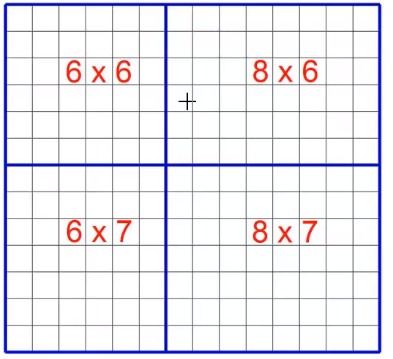
\includegraphics[width=5cm]{../images/20210421/ej1_1}}
\hfill
\subfigure[Área de influencia de nudos]{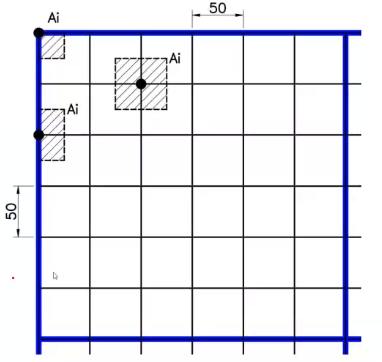
\includegraphics[width=5cm]{../images/20210421/ej1_2}}
\hfill
\end{figure}

Donde hay que hacer una corrección, donde la grilla de la esquina superior derecha,
donde en realidad la grillas superiores tienen que ser iguales a las inferiores
y las inferiores a las superiores, ya que consideramos una distancia de $\SI{0.5}{m}$.

Luego, encontramos una \textit{aproximación} al comportamiento de cuasi-resorte
del suelo a partir delc oeficiente de balasto de la siguiente forma:

\begin{align*}
  K_r = b * \frac{1}{2} * (\Delta_1 + \Delta_2 ) *K_s
.\end{align*}

\textbf{Rigidez de los apoyos interiores}

Analizando la figura de área de influencia, podemos ver que los elementos tendrán
las áreas mostradas, por lo que las rigideces serán:

\begin{align*}
  k_r &= k_s * A_i = \SI{5}{t / cm} \hspace{0.25cm} \xrightarrow{\hspace*{0.5cm}} \hspace{0.1cm} \text{Rigidez de apoyo interior} \\[5pt]
  k_r &= k_s * A_i = \SI{2.5}{t / cm} \hspace{0.25cm} \xrightarrow{\hspace*{0.5cm}} \hspace{0.1cm} \text{Rigidez de apoyo de borde}  \\[5pt]
  k_r &= k_s * A_i = \SI{1.25}{t /cm} \hspace{0.25cm} \xrightarrow{\hspace*{0.5cm}} \hspace{0.1cm} \text{Rigidez de apoyo de esquina} 
.\end{align*}

Seguimos con RAM para la formación de una placa. Primero definimos los puntos,
luego las unimos con vigas, y por último las unimos con placas. El modelo será
algo similar a lo referenciado en \Cref{fig:ej1_ram1}.

\begin{figure}[htpb]
  \centering
  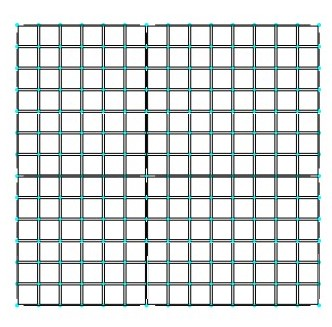
\includegraphics[width=0.5\textwidth]{../images/20210421/ej1_ram1}
  \caption{Modelo de RAM Elements}
  \label{fig:ej1-ram1}
\end{figure}

Luego, debemos darle dimensiones a las vigas, que en nuestro caso adoptamos
vigas de 50x90cm, y en los apoyos, debemos darle \textbf{restricciones elásticas},
donde utilizaremos los valores encontrados para cada tipo de apoyo. Podemos cambiar
el tipo de unidad del programa a \textit{Métrico} para poder utilizar las unidades
de t/cm obtenidos.

Luego de cargados estos datos, podemos hacer el análisis de elementos finitos. 
\end{document}
